\documentclass[12pt,a4paper]{article}

% Packages
\usepackage[utf8]{inputenc}
\usepackage{amsmath, amssymb}
\usepackage[a4paper,
  top=1in,
  bottom=1in,
  left=1.25in,
  right=1in]{geometry}
\usepackage{graphicx}
\usepackage{hyperref}
\usepackage{setspace}
\usepackage{titlesec}

\begin{document}

%========================
% Title Page
%========================
\begin{titlepage}
    \thispagestyle{empty}
    \centering
    \vspace*{\fill}

    {\Huge \textbf{On the Proximity of Cosmic}}\\[0.2cm]
    {\Huge \textbf{Mass--Radius Ratios to}}\\[0.4cm]
    {\Huge \textbf{Black Hole Limits}}\\[0.6cm]

    {\LARGE Vinayak Ghai}\\[0.5cm]
    {\Large Independent Research Project}\\[1cm]
    {\Large \today}

    \vspace*{\fill}
\end{titlepage}

\newpage

%========================
% Abstract
%========================
\begin{abstract}

This study examines how the masses and radii of astrophysical objects relate to the extreme limits associated with black hole formation. Black holes are characterized by a critical geometric boundary known as the Schwarzschild radius, beyond which spacetime curvature prevents causal escape. While this boundary is sharply defined within general relativity, it is often tempting to apply Schwarzschild-based reasoning to ordinary cosmic objects using simplified Newtonian intuition.

We begin by exploring such naive mass--radius comparisons and demonstrate how mathematically valid arguments can become physically misleading when relativistic structure and internal pressure are ignored. To clarify this distinction, we introduce a heuristic kinematic timescale derived through dimensional reasoning and compare it with the relativistic characteristic timescale naturally associated with black hole horizons.

The analysis highlights how dimensional consistency and geometric scaling can reproduce correct orders of magnitude even within simplified models, while emphasizing that numerical agreement does not imply physical equivalence. This work aims to clarify the boundary between intuition and rigor in gravitational physics and to illustrate how physical meaning emerges only when mathematical expressions are interpreted within their proper theoretical context.

\end{abstract}

\newpage

%========================
% Introduction
%========================
\section{Introduction}

\subsection{Background and Motivation}

The Schwarzschild radius arises in general relativity as a fundamental geometric scale associated with gravitational collapse. For a spherically symmetric mass $M$, it is given by
\begin{equation}
r_s = \frac{2GM}{c^2},
\end{equation}
where $G$ is the gravitational constant and $c$ is the speed of light. This radius defines the location of the event horizon for a non-rotating black hole.

Because of its simple algebraic form, the Schwarzschild condition is frequently rewritten as a mass--radius inequality and applied to objects far from relativistic collapse. Such reformulations often originate from Newtonian escape velocity arguments, which suggest that collapse occurs when the escape speed reaches $c$. While this intuition is mathematically suggestive, it obscures the fundamentally geometric origin of the Schwarzschild radius.

This tension between mathematical simplicity and physical meaning motivates the present work.

\subsection{Limitations of Naive Schwarzschild Arguments}

In Newtonian gravity, the escape velocity from a body of mass $M$ and radius $R$ is
\begin{equation}
v_{\text{esc}} = \sqrt{\frac{2GM}{R}}.
\end{equation}
Formally setting $v_{\text{esc}} = c$ yields
\begin{equation}
R = \frac{2GM}{c^2},
\end{equation}
which matches the Schwarzschild radius.

However, this derivation neglects spacetime curvature, relativistic pressure, and the internal equation of state of matter. As a result, it can suggest physically impossible scenarios when applied to ordinary stars or planets. The Schwarzschild radius is not a Newtonian collapse condition, but a relativistic causal boundary.

\subsection{Scope and Aim of This Work}

This paper investigates how far simplified, Newtonian-inspired reasoning can be extended before it loses physical meaning. Rather than attempting to model black hole interiors or horizon dynamics, we focus on the emergence of characteristic scales and times through dimensional analysis and geometric reasoning.

\begin{figure}[ht!]
    \centering
    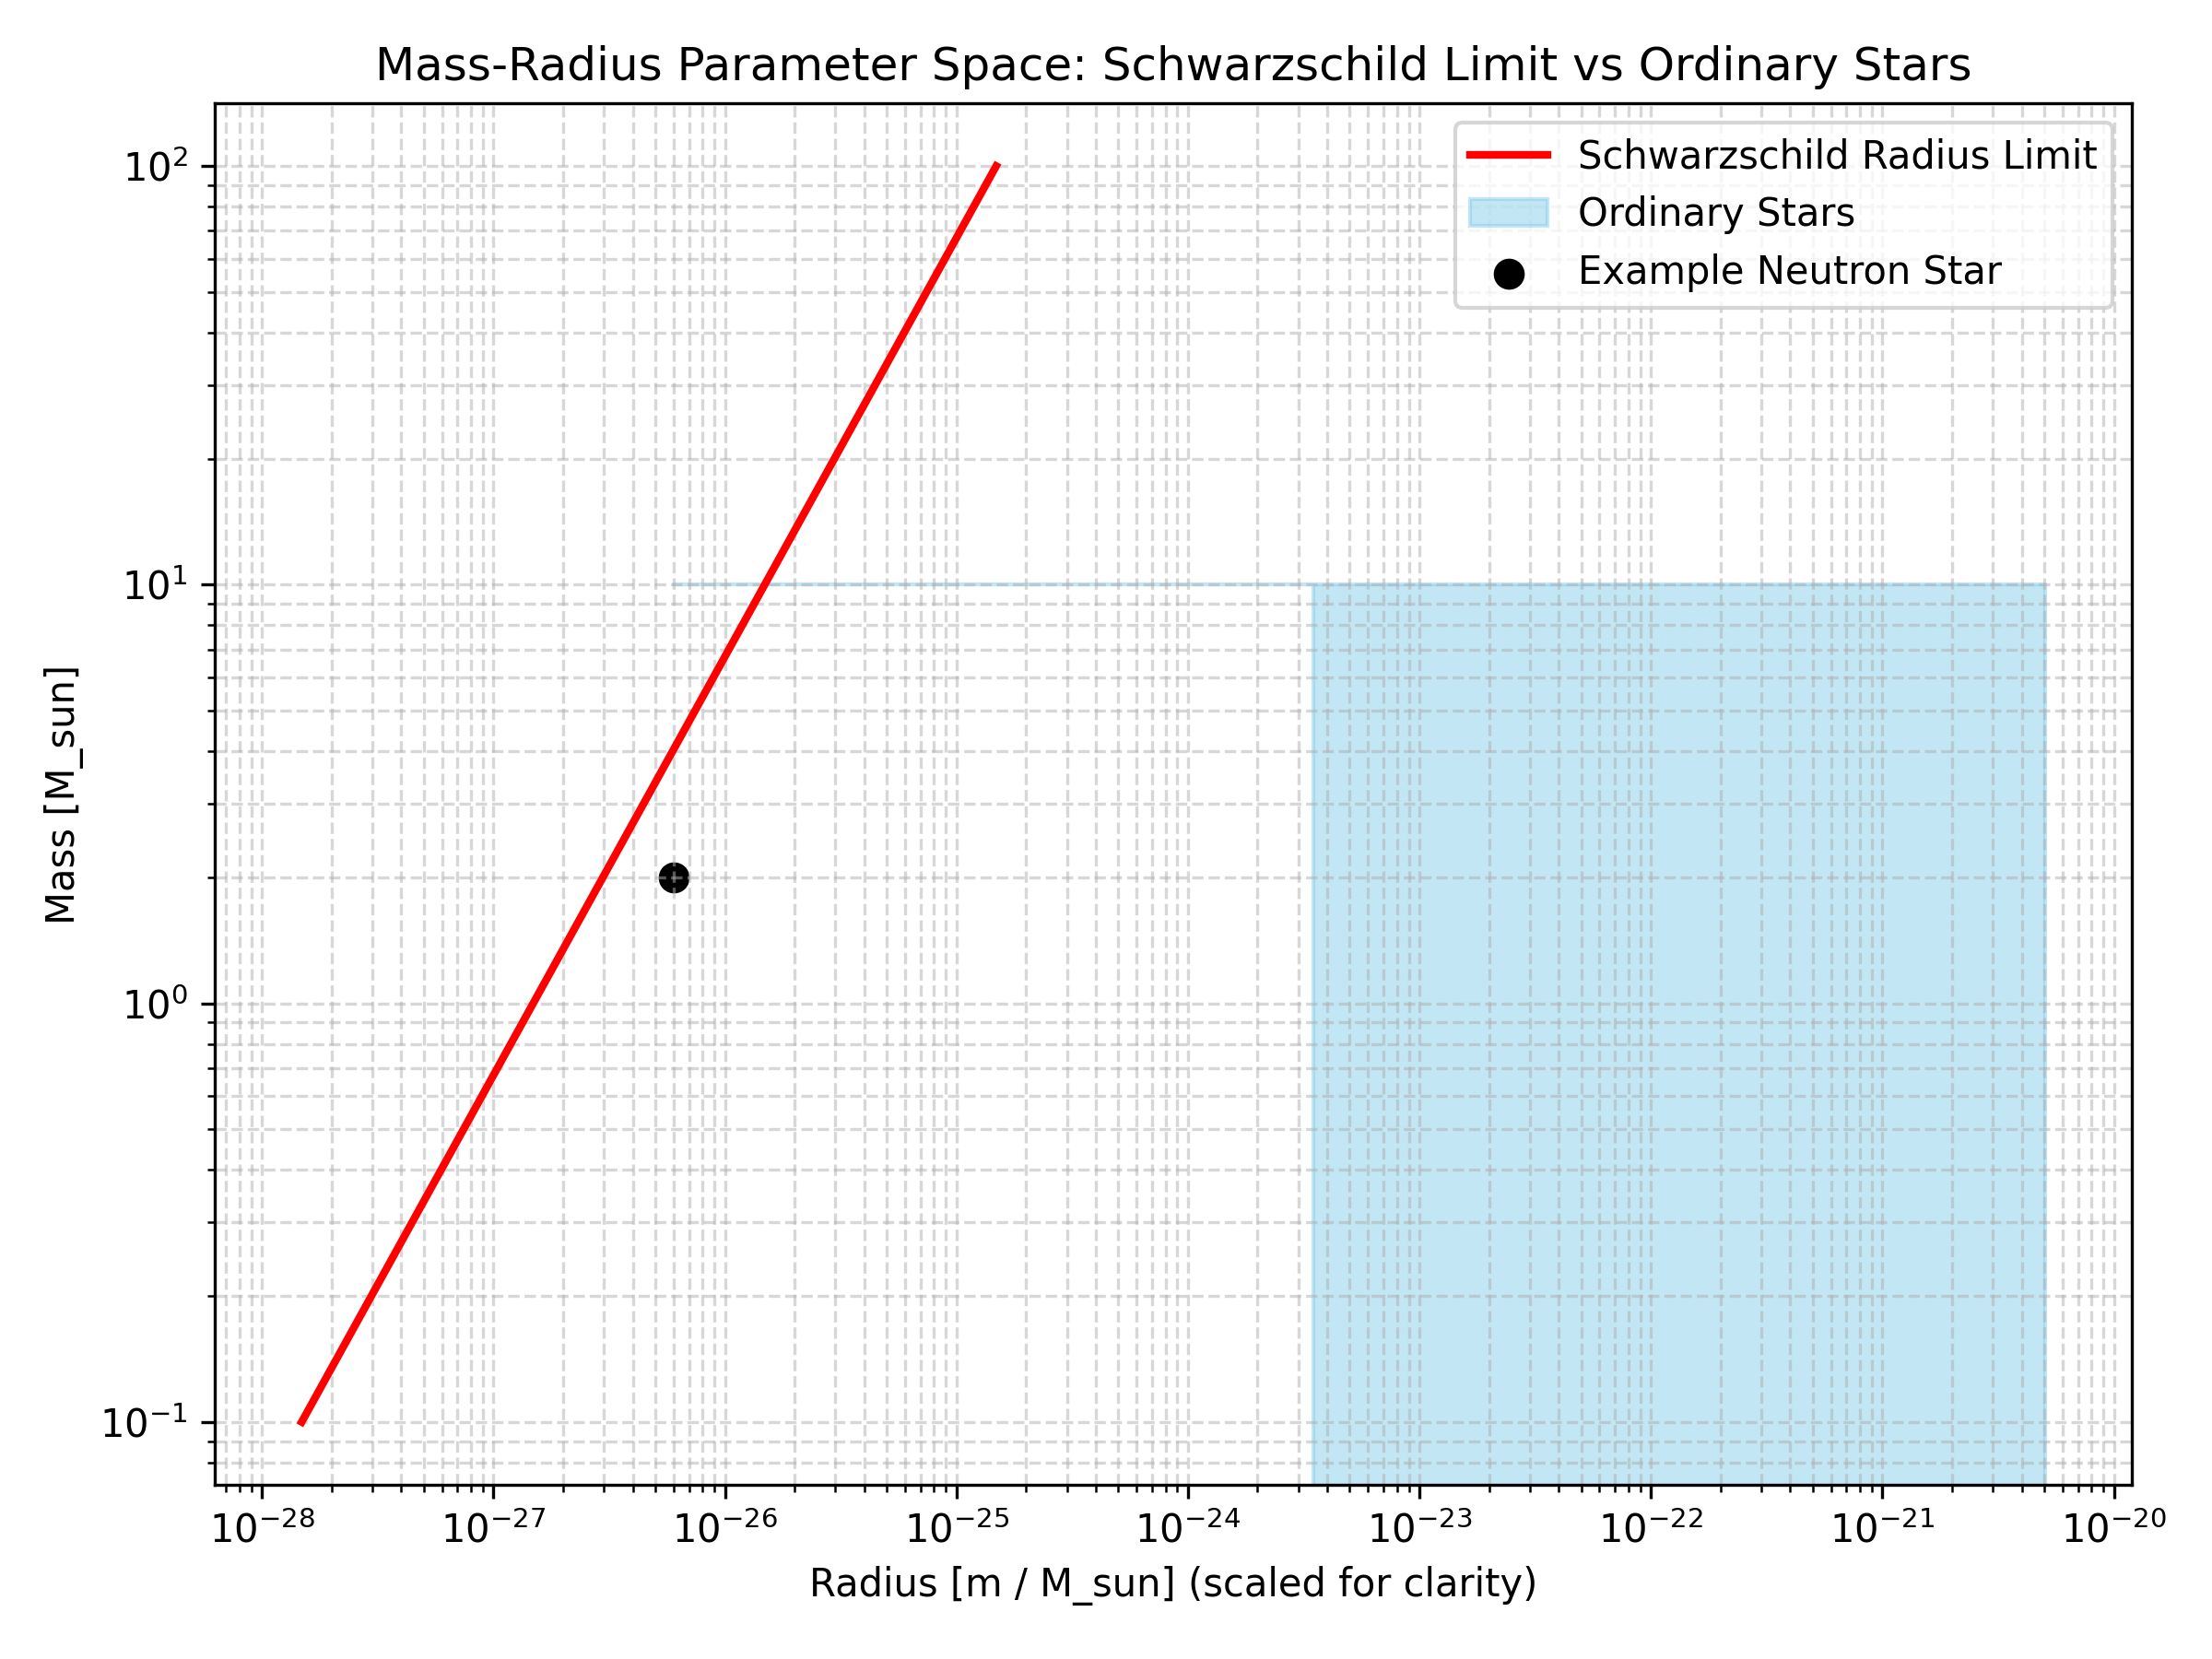
\includegraphics[width=0.7\textwidth]{figures/mass_radius_diagram.png}
    \caption{Mass--radius parameter space illustrating the Schwarzschild boundary (red line). Ordinary stars and planets lie far below this limit, emphasizing the gap between Newtonian intuition and relativistic collapse.}
    \label{fig:mass-radius}
\end{figure}

%========================
% Heuristic Reformulation
%========================
\section{A Heuristic Reformulation of the Schwarzschild Condition}

\subsection{Algebraic Structure}

The Schwarzschild condition may be written as
\begin{equation}
\frac{2GM}{R} = c^2,
\end{equation}
or equivalently,
\begin{equation}
2GM = c^2 R.
\end{equation}

At this stage, it is tempting to introduce kinematic interpretations involving motion at speed $c$. We emphasize that the following manipulation is \emph{purely heuristic} and is not intended to describe any physically realizable trajectory in curved spacetime.

Formally writing one factor of $c$ as
\begin{equation}
c = \frac{dx}{dt},
\end{equation}
we obtain
\begin{equation}
2GM = c R \frac{dx}{dt}.
\end{equation}

Multiplying both sides by $dt$ yields
\begin{equation}
2GM\, dt = c R\, dx.
\label{eq:heuristic}
\end{equation}

Equation~\eqref{eq:heuristic} is algebraically valid and dimensionally consistent, but it carries no direct physical interpretation within general relativity.

\subsection{Heuristic Integration and Emergent Timescale}

Integrating Equation~\eqref{eq:heuristic} over finite intervals gives
\begin{equation}
\int 2GM\, dt = \int c R\, dx,
\end{equation}
leading to
\begin{equation}
2GM\, T = c R\, x,
\end{equation}
where $T$ represents a formally constructed traversal time associated with a coordinate distance $x$.

Rearranging,
\begin{equation}
T = \frac{c R x}{2GM}.
\end{equation}

At this stage, the expression remains entirely heuristic. Its purpose is not physical realism, but comparison with relativistically meaningful timescales.

%========================
% Relativistic Timescale
%========================
\section{Relativistic Characteristic Timescale}

In general relativity, the Schwarzschild radius
\begin{equation}
r_g = \frac{2GM}{c^2}
\end{equation}
defines a fundamental geometric length scale. Dividing by $c$ yields a natural relativistic timescale,
\begin{equation}
\tau = \frac{r_g}{c} = \frac{2GM}{c^3}.
\end{equation}

This timescale sets the order of magnitude for the fastest possible processes occurring near a black hole horizon and is widely used in relativistic astrophysics.

%========================
% Integrated Traversal Time
%========================
\section{Integrated Traversal Time}

The Integrated Traversal Time $\Lambda$ constitutes a fundamental quantity arising from the naive kinematic integration presented earlier. While this framework is heuristic in nature—neglecting gravitational redshift, coordinate singularities, and genuine horizon dynamics—it provides a structured and interpretable measure of path-dependent traversal durations within the simplified model.

\subsection{Formulation of the Integrated Traversal Time}

Starting from the integration, we have
\begin{equation}
4GM \, T = c \, R \, x,
\end{equation}
where $x$ denotes the radial coordinate interval traversed, and $R$ is the characteristic radius.

Substituting the Schwarzschild radius $R = 2GM/c^2$ yields
\begin{equation}
4GM \, T = c \left(\frac{2GM}{c^2}\right) x = \frac{2GM}{c} x.
\end{equation}

Dividing both sides by $4GM$ isolates the traversal timescale:
\begin{equation}
T = \frac{x}{2c}.
\end{equation}

We now formally redefine this quantity as
\begin{equation}
\Lambda \equiv T = \frac{x}{2c},
\end{equation}
the \textbf{Integrated Traversal Time}.

\subsection{Horizon-Scale Comparison}

To compare $\Lambda$ and $\tau$ directly, we set the traversal distance $x$ equal to the diameter of the black hole event horizon:
\begin{equation}
x = 2r_g
\end{equation}

Substituting into $\Lambda$:
\begin{equation}
\Lambda = \frac{2r_g}{2c} = \frac{r_g}{c} = \tau
\end{equation}

Thus, at the horizon scale, $\Lambda = \tau$.

\subsection{Scaling Across Mass Regimes}

Table~\ref{table:timescales} compares the timescales.

\begin{table}[h!]
\centering
\begin{tabular}{|c|c|c|c|}
\hline
\textbf{Black Hole Type} & \textbf{Mass ($M$)} & \textbf{Relativistic $\tau$} & \textbf{Integrated $\Lambda$ ($x = 2r_g$)} \\
\hline
Stellar-mass & $10\,M_\odot$ & $\sim 50\,\mu\text{s}$ & $\sim 50\,\mu\text{s}$ \\
Intermediate-mass & $10^4\,M_\odot$ & $\sim 0.05\,\text{s}$ & $\sim 0.05\,\text{s}$ \\
Supermassive & $10^9\,M_\odot$ & $\sim 1.5\,\text{hours}$ & $\sim 1.5\,\text{hours}$ \\
\hline
\end{tabular}
\caption{Comparison of timescales.}
\label{table:timescales}
\end{table}

\subsection{Refined Interpretation}

The Integrated Traversal Time $\Lambda$ represents a dimensionally consistent timescale. Its numerical agreement with $\tau$ at horizon-scale distances is noteworthy, yet it does not signify that $\Lambda$ captures genuine relativistic dynamics.

\subsubsection{Understanding the Distinction through Analogies}

Analogies help clarify: the ruler and the road, the menu and the meal, the shadow and the object.

\subsubsection{Reconciling Agreement and Distinction}

This framework highlights the interplay between dimensional consistency and physical interpretation. The agreement between $\Lambda$ and $\tau$ demonstrates that elementary constructs can reproduce correct orders of magnitude.

In summary: $\Lambda$ is to $\tau$ what a map is to a territory.

%========================
% Conclusion
%========================
\section{Conclusion}

This work has explored the boundaries between Newtonian intuition and relativistic rigor in gravitational physics. By examining naive mass-radius comparisons and heuristic kinematic timescales, we have demonstrated how dimensional consistency can lead to correct orders of magnitude even in simplified models.

The key insight is that numerical agreement does not imply physical equivalence. The Schwarzschild radius and its associated timescales provide geometric and temporal scales that emerge consistently across different frameworks, but their interpretation requires careful consideration of the underlying physics.

Future work could extend this analysis to rotating black holes or incorporate quantum effects near the Planck scale.

\bibliographystyle{plain}
\bibliography{references}

\end{document}
